\chapter{Introduction to Graph Theory}

\section{Introduction}

A graph consists of a nonempty set V of vertices and a set E of edges, where each edge in E connects two (may be the same) vertices in V.

We usually use \(G = (V, E)\) to indicate the above relationship.

Furthermore, if each edge connects two different vertices, and no two edges connect the same pair of vertices, then the graph is a simple graph. For example, the graph below is a simple graph.

\begin{figure}[H]
  \centering
  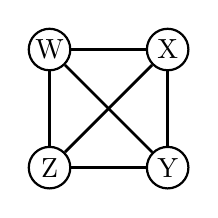
\begin{tikzpicture}[node distance={15mm}, thick, main/.style = {draw, circle}]
    \centering
    \tikzstyle{vertex}=[circle,draw=black,thick,fill=white,minimum size=15pt, inner sep=0pt]
    \node[vertex] (Z) at (0, 0) {Z};
    \node[vertex] (W) at (0, 1.5) {W};
    \node[vertex] (X) at (1.5, 1.5) {X};
    \node[vertex] (Y) at (1.5, 0) {Y};
    \path[every node/.style={font=\sffamily\small},line width=1pt]
    (Z) edge (W) 
    (W) edge (X) 
    (X) edge (Y) 
    (Y) edge (Z)
    (W) edge (Y)
    (Z) edge (X)
    ;
  \end{tikzpicture}
  \quad\quad\quad
  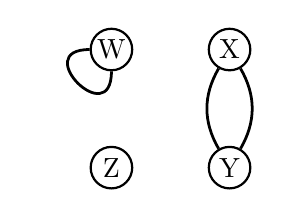
\begin{tikzpicture}[node distance={15mm}, thick, main/.style = {draw, circle}]
    \centering
    \tikzstyle{vertex}=[circle,draw=black,thick,fill=white,minimum size=15pt, inner sep=0pt]
    \node[vertex] (Z) at (0, 0) {Z};
    \node[vertex] (W) at (0, 1.5) {W};
    \node[vertex] (X) at (1.5, 1.5) {X};
    \node[vertex] (Y) at (1.5, 0) {Y};
    \path[every node/.style={font=\sffamily\small},line width=1pt]
    (W) edge [out=180,in=270,looseness=5] (W)
    (X) edge [bend left] (Y)
    (X) edge [bend right] (Y)
    ;
  \end{tikzpicture}
\end{figure}